\section{Normed spaces}
\label{sec:normed-banach-spaces}

\subsection{As special metric spaces}

\begin{defn}
  \label{def:ambientMetricSpace}
  The \emph{ambient metric space} of a normed space $(V, \|\cdot\|)$
  is the metric space $(V, d)$
  where the metric $d$ is given by
  $d(x,y) = \|x-y\|$.
\end{defn}

\begin{exc}
  Show that the ambient metric space is indeed a metric space.
\end{exc}

\begin{defn}%[Convergence of sequences]
  \label{def:convergenceNormedSpace}
  A sequence $(u_n)$ in a normed space $(V, \|\cdot\|)$
  is \emph{convergent} to $u$
  iff $(u_n)$ converges to $u$
  in the ambient complete metric space
  as in Definition \ref{def:convergenceOfSequenceMetricSpace}.
\end{defn}

\begin{lem}
  \label{lem:openBallsAreConvex}
  Any open ball in a normed space is a convex set,
  c.f. Definitions \ref{def:convexFunc} and \ref{def:openBallMetricSpace}.
\end{lem}

\begin{exm}
  \label{exm:notEuclidNormIfLess1}
  Consider the complementary case to Example \ref{exm:RdEuclideanSpace}:
  is $\left(\mathbb{R}^n, \|\cdot\|_p\right)$
  a normed space for $p\in(0,1)$?
  By Lemma \ref{lem:openBallsAreConvex},
  it is not a norm if any open ball is not convex.
  For $p=\frac{1}{2}$,
  the boundary of the open ball
  $\{\mathbf{x}: \|\mathbf{x}\|_{\frac{1}{2}}<1\}$ with
  $\|\mathbf{x}\|_{\frac{1}{2}}:=\left(\sqrt{x_1}+\sqrt{x_2}\right)^2$
  shown in Figure \ref{fig:notANormIfpLessThan1} bounds a concave region 
  and hence $\|\cdot\|_p$ is not a norm for $p\in(0,1)$.
\end{exm}

\begin{Figure}
  \centering
  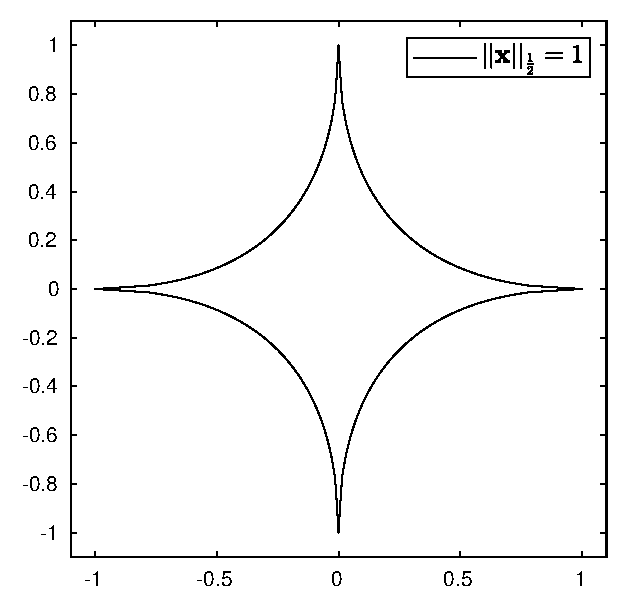
\includegraphics[width=0.6\linewidth]{eps/UnitBallNorm05}
  \captionof{figure}{$\left(\mathbb{R}^n, \|\cdot\|_p\right)$
    with $p\in(0,1)$ is not a normed space. 
  }
  \label{fig:notANormIfpLessThan1}
\end{Figure}

\begin{defn}
  \label{def:normsOfContFuncs}
  Let $\Omega\subset \mathbb{R}^n$ be a bounded open set.
  The \emph{$p$-norm of a continuous scalar function} in the linear space
  ${\cal C}(\overline{\Omega})$
  is 
  \begin{equation}
    \label{eq:pNormOfContFuncs}
    \forall v\in {\cal C}(\overline{\Omega}),\quad
    \|v\|_p :=  \left[\int_{\Omega}|v(\mathbf{x})|^p
      \dif \mathbf{x}\right]^{\frac{1}{p}}
  \end{equation}
  and the \emph{$\infty$-norm} or \emph{maximum norm}
  is given by 
  \begin{equation}
    \label{eq:maxNormOfContFuncs}
    \forall v\in {\cal C}(\overline{\Omega}),\quad
    \|v\|_{\infty} :=  \max_{\mathbf{x}\in \overline{\Omega}}
    |v(\mathbf{x})|.
  \end{equation}
\end{defn}

\begin{exm}
  $({\cal C}(\overline{\Omega}), \|\cdot\|_{\infty})$
  in Definition \ref{def:normsOfContFuncs} 
  is a normed space,
  so is $({\cal C}(\overline{\Omega}), \|\cdot\|_{p})$
  for any $p\in [1,\infty)$.
\end{exm}

\begin{exm}
  For the $\ell^{\infty}$ sequence space in (\ref{eq:ellInftySpace}), 
  \begin{displaymath}
    \ell^{\infty} := \left\{
      (a_n)_{n\in \mathbb{N}}: \sup_{n\in \mathbb{N}}|a_n| < \infty.
    \right\},
  \end{displaymath}
  define $\|\cdot\|_{\infty}: \ell^{\infty}\rightarrow \mathbb{R}^+\cup\{0\}$ as
  \begin{equation}
    \label{eq:ellInftyNorm}
    \left\|(a_n)_{n\in \mathbb{N}}\right\|_{\infty}
    = \sup_{n\in \mathbb{N}} |a_n|.
  \end{equation}
  Then $(\ell^{\infty}, \|\cdot\|_{\infty})$
  is a normed space.
\end{exm}

\begin{exm}
  For the $\ell^{p}$ space in (\ref{eq:lpSpace})
  with $p\in [1,\infty)$,
  \begin{displaymath}
    \ell^p := \left\{
      (a_n)_{n\in \mathbb{N}}: a_n\in \mathbb{C};
      \sum_{n\in \mathbb{N}} |a_n|^p < \infty
    \right\}, 
  \end{displaymath}
  we have
  \begin{align*}
     &\left\{
    \begin{array}{l}
      (a_n)_{n\in \mathbb{N}}\in \ell^p, \  
      (b_n)_{n\in \mathbb{N}}\in \ell^p
    \\
      |a+b|^p \le (|a|+|b|)^p \le 2^p(\max(|a|,|b|))^p
                  \le 2^p(|a|^p+|b|^p)
    \end{array}
    \right.
    \\
    &\Rightarrow
     (a_n)_{n\in \mathbb{N}}+(b_n)_{n\in \mathbb{N}}\in \ell^p,
  \end{align*}
  where the comparison test is applied.

  Then $(\ell^{p}, \|\cdot\|_{p})$
  is a normed space where
  \begin{equation}
    \label{eq:ellPNorm}
    \left\|(a_n)_{n\in \mathbb{N}^+}\right\|_p
    := \left(\sum_{n=1}^{\infty} |a_n|^p\right)^{\frac{1}{p}}.
  \end{equation}
\end{exm}

\subsection{Continuous maps of normed spaces}

\begin{lem}
  \label{lem:normIsContinuousMap}
  The norm function $\|\cdot\|$ is continuous.
\end{lem}

\begin{lem}
  \label{lem:monotonicityOfEuclideanNorm}
  The Euclidean norm $\|\cdot\|_p$
  in Example \ref{exm:RdEuclideanSpace}
  satisfies a monotonicity property:
  \begin{equation}
    \label{eq:monotonicityOfEuclideanNorm}
    1\le p \le q \le \infty
    \ \Rightarrow\
    \forall \mathbf{x}\in \mathbb{R}^n\ 
    \|\mathbf{x}\|_q \le \|\mathbf{x}\|_p.
  \end{equation}
\end{lem}

\begin{exm}
  The map $S: ({\cal C}[0,1], \|\cdot\|_{\infty}) \rightarrow
  (\mathbb{R}, |\cdot|)$,  
  \begin{equation}
    \label{eq:contFunExmpInt}
    S(f) = \int_0^1 f^2(x) \dif x, 
  \end{equation}
  is continuous.
  Indeed, for any $g\in {\cal C}[0,1]$, 
  we have
  \begin{align*}
    |S(f)-S(g)| &= 
    \left| \int_0^1 f^2(x) \dif x - \int_0^1 g^2(x) \dif x
                  \right|
    \\ &\le
         \int_0^1 \left|f(x)-g(x)\right|
                  \left|f(x)-g(x)+2g(x)\right|
         \dif x 
    \\ &\le
         \int_0^1 \left\|f-g\right\|_{\infty}
         \left(\left\|f-g\right\|_{\infty}+2\|g\|_{\infty}\right)
         \dif x, 
  \end{align*}
  which yields  
  \begin{align*}
    &\forall \epsilon>0,
    \exists \delta=\min\left(1,\frac{\epsilon}{1+2\|g\|_{\infty}}\right)
      \text{ s.t. }
    \|f-g\|_{\infty} < \delta\ \Rightarrow\
    \\
    & \left\|f-g\right\|_{\infty}
      \left(\left\|f-g\right\|_{\infty}+2\|g\|_{\infty}\right)
      <
      \left\|f-g\right\|_{\infty}
      \left(1+2\|g\|_{\infty}\right)
      < \epsilon
    \\
    & \Rightarrow\ |S(f)-S(g)| <\epsilon.
  \end{align*}
\end{exm}

\begin{exc}
  For $V={\cal C}[0,1]$ and $x_0\in [0,1]$,
  define $\ell_{x_0}: V\rightarrow \mathbb{R}$ as
  $\ell_{x_0}(v) := v(x_0)$.
  Show that $\ell_{x_0}$ is continuous on ${\cal C}[0,1]$.
\end{exc}

\begin{exm}
  \label{exm:continuityOfDifferentiation}
  The differentiation map
  \begin{displaymath}
    \frac{\dif}{\dif t}:
    ({\cal C}^1[a,b],\|\cdot\|_{\infty})
    \rightarrow ({\cal C}[a,b], \|\cdot\|_{\infty})
  \end{displaymath}
  is not continuous, but can be made
  continuous if we change the norm on ${\cal C}^1[a,b]$ to
  \begin{equation}
    \label{eq:normForC1}
    \|f\|_{1,\infty}:= \|f\|_{\infty} + \|f'\|_{\infty}.
  \end{equation}
  Indeed,
  for $f_n(t) = \frac{1}{\sqrt{n}}\cos(2\pi nt)$,
  we have
  \begin{align*}
    \forall n\in \mathbb{N}^+,\quad
    \|f'_n-\mathbf{0}'\|_{\infty} = 2\pi\sqrt{n} > 1, 
  \end{align*}
  yet $\|f_n-\mathbf{0}\|$ can be made arbitrarily small
  as $n \rightarrow \infty$.
  In contrast,
  $D: ({\cal C}^1[a,b],\|\cdot\|_{1,\infty})
  \rightarrow ({\cal C}[a,b], \|\cdot\|_{\infty})$ is continuous because
  \begin{align*}
    &\forall \epsilon>0,\ \exists \delta=\epsilon, \text{ s.t. }\ 
      \forall f,g\in {\cal C}^1[0,1],\ 
      \|f - g\|_{1,\infty}<\delta
    \ \Rightarrow\ 
    \\
    &
    \|Df - Dg\|_{\infty}
    = \|f' - g'\|_{\infty} \le
    \|f - g\|_{1,\infty} < \delta=\epsilon.
  \end{align*}
\end{exm}

\begin{exc}
  \label{exc:arcLengthFunctionNotContinuous}
  Show that the arc length function $L: {\cal C}^1[0,1]\rightarrow\mathbb{R}$,
  \begin{equation}
    \label{eq:arcLengthFunction}
    L(f) := \int_0^1 \sqrt{1+(f'(t))^2} \dif t,
  \end{equation}
  is not continuous if the norm of ${\cal C}^1[0,1]$ is
  $\|\cdot\|_{\infty}$,
  whereas it is continuous if we equip ${\cal C}^1[0,1]$ with
  (\ref{eq:normForC1}).
\end{exc}

\begin{exc}
  Is the function
  $S: (c_{00}, \|\cdot\|_{\infty}) \rightarrow (\mathbb{R}, |\cdot|)$,
  \begin{equation}
    \label{eq:c00FuncNotCont}
    S\left((a_n)_{n\in \mathbb{N}}\right) = \sum_{n=1}^{\infty} a_n^2
  \end{equation}
  continuous?
  Here $c_{00}$ is defined in Notation \ref{ntn:zeroSequenceSpaces}. 
\end{exc}

\subsection{Norm equivalence}
\label{sec:norm-equivalence}

\begin{defn}
  \label{def:equivalentNorms}
  Two norms $\|\cdot\|_A$ and $\|\cdot\|_B$ on $V$ are
  \emph{equivalent}, written $\|\cdot\|_A\sim \|\cdot\|_B$, iff
  \begin{equation}
    \label{eq:equivalentNorms}
    \exists c_1, c_2\in \mathbb{R}^+ \text{ s.t. }
    \forall v\in V,\quad
    c_1\|v\|_A \le \|v\|_B \le c_2 \|v\|_A.
  \end{equation}
\end{defn}

\begin{exm}
  The Euclidean norms in Definition \ref{def:EuclideanLpNorm}
  satisfy
  \begin{equation}
    \label{eq:EuclideanNormsAreEquivalent}
    \forall \mathbf{x} \in \mathbb{R}^n,\quad
    \|\mathbf{x}\|_{\infty} \le \|\mathbf{x}\|_p
    \le \sqrt[p]{n} \|\mathbf{x}\|_{\infty}.
  \end{equation}
  Therefore all the Euclidean $\ell_p$ norms
  are equivalent.
\end{exm}

\begin{exm}
  The operator norm and the Hilbert-Schmidt norm
  in Definitions \ref{def:operatorNorm}
  and \ref{def:HilbertSchmidtNorm}
  are equivalent. 
\end{exm}

\begin{exc}
  \label{exc:equivalenceOfNorms}
  Show that $\sim$ in Definition \ref{def:equivalentNorms}
  defines an equivalence relation
  on the set of all norms on $V$.
\end{exc}

\begin{lem}
  \label{lem:normEquivCondViaConvergence}
  Show that two norms $\|\cdot\|_A$ and $\|\cdot\|_B$
  on a linear space $V$ are equivalent
  if and only if each sequence converging with respect to
  one norm %$\|\cdot\|_A$
  also converges with respect to the other. %$\|\cdot\|_B$.
\end{lem}

\begin{thm}
  \label{thm:normEquivalenceRn}
  All norms are equivalent on $\mathbb{R}^n$ or $\mathbb{C}^n$.
\end{thm}

\begin{coro}
  \label{coro:normEquivalenceFiniteDim}
  Over a finite-dimensional space,
  any two norms are equivalent.
\end{coro}

\begin{exm}
  In the normed space $V:= {\cal C}[0,1]$, 
  consider a sequence of functions
  $(u_n)$ given by
  \begin{displaymath}
    u_n(x) :=
    \begin{cases}
      1-nx, & x\in [0,\frac{1}{n}];
      \\
      0, & x\in (\frac{1}{n}, 1].
    \end{cases}
  \end{displaymath}
  For the $p$-norm in (\ref{eq:pNormOfContFuncs}),
  we have $\|u_n\|_p = [n(p+1)]^{-\frac{1}{p}}$
  and thus the sequence $(u_n)$ converges
  to $u=0$ in $(V,\|\cdot\|_p)$.
  However, for the $\infty$-norm in (\ref{eq:maxNormOfContFuncs}),
  we have $\|u_n\|_{\infty} = 1$.
  By Definition \ref{def:equivalentNorms}, 
  these two norms can not be equivalent. 
\end{exm}

\subsection{Completeness}

\begin{defn}[Banach spaces]
  \label{def:BanachSpace}  
  A \emph{Banach space} is a \emph{complete} normed space, 
  i.e., a normed space $V$ such that
  every Cauchy sequence in $V$ converges in $V$.
\end{defn}

\begin{defn}
  A \emph{Hilbert space} is a Banach space equipped with an inner product.
\end{defn}

\begin{thm}
  \label{thm:contFuncWithInftyNormIsComplete}
  $\left({\cal C}[a,b], \|\cdot\|_{\infty}\right)$
  is a Banach space.
\end{thm}

\begin{exm}
  \label{exm:CpIsNotComplete}
  For $p\in[1,\infty)$, 
  the space $\left({\cal C}(\overline{\Omega}), \|\cdot\|_{p}\right)$
  is not a Banach space. 
  Consider % $\Omega=[0,1]$ and
  $\left(u_n\right)_{n\in \mathbb{N}}\subset
  {\cal C}[0,1]$
  given by
  \begin{equation}
    \label{eq:CpIsNotComplete}
    u_n(x) =
    \begin{cases}
      0, & x\in [0,\frac{1}{2}-\frac{1}{2n}];
      \\
      nx - \frac{n-1}{2}, & x\in [\frac{1}{2}-\frac{1}{2n},
      \frac{1}{2}+\frac{1}{2n}];
      \\
      1 & x\in [\frac{1}{2}+\frac{1}{2n},1].
    \end{cases}
  \end{equation}
  $(u_n)_{n\in \mathbb{N}}$ is clearly Cauchy
  and we have
  \begin{displaymath}
    \lim_{n\rightarrow \infty} u_n = u(x) =
    \begin{cases}
      0, & x\in [0, \frac{1}{2});
      \\
      1, & x\in (\frac{1}{2}, 1].
    \end{cases}
  \end{displaymath}
  But $u(x)$ cannot be in ${\cal C}(\overline{\Omega})$
  no matter how we define $u(\frac{1}{2})$.
\end{exm}

\begin{defn}
  \label{def:isomorphicN0ormedSpaces}
  Two normed spaces $X$ and $Y$
  are \emph{isomorphic}, written $X\simeq Y$, 
  iff there exists a bijective linear map
  $T\in {\cal L}(X, Y)$ such that
  \begin{equation}
    \label{eq:isometricIsomorphism}
    \forall v\in X,\quad \|T v\|_Y = \|v\|_X.
  \end{equation}
  Then $T$ is an \emph{(isometric) isomorphism}
  between $X$ and $Y$.
\end{defn}

\begin{thm}
  \label{thm:completionOfNormedSpace}
  Every normed space $V$ has a unique \emph{completion}
  up to isometric isomorphism,
  i.e., 
  there exists a unique Banach space $W$
  such that $V$ is isomorphic to a dense subspace of $W$.
\end{thm}

\begin{defn}
  \label{def:completionOfNormedSpace}
  The Banach space $W$ in Theorem \ref{thm:completionOfNormedSpace}
  is called the \emph{completion of the normed space} $V$.  
\end{defn}

\begin{exc}
  \label{exc:ellInftyComplete}
  Show that the sequence space
  $(\ell^{\infty}, \|\cdot\|_{\infty})$ is complete.
\end{exc}

\begin{exc}
  Define ${\cal C}_b[0,\infty)$ as the set of all functions
  $f$ that are continuous on $[0,\infty)$
  and satisfy
  \begin{displaymath}
    \|f\|_{\infty} := \sup_{x\ge 0}|f(x)| < \infty.
  \end{displaymath}
  Show ${\cal C}_b[0,\infty)$ with this norm is complete.
\end{exc}

\begin{exc}
  Define ${\cal C}^{\alpha}[a,b]$ as the set of all functions
  $f\in {\cal C}[a,b]$ satisfying
  \begin{displaymath}
    M_{\alpha}(f) := \sup_{x,y\in[a,b]; x\ne y}
    \frac{|f(x)-f(y)|}{|x-y|^{\alpha}} < \infty.
  \end{displaymath}
  Define $\|f\|_{\alpha} := \|f\|_{\infty}+M_{\alpha}(f)$.
  Show that $({\cal C}^{\alpha}[a,b], \|\cdot\|_{\alpha})$
  is a Banach space.
\end{exc}

\subsection{Convergence of function series}

\begin{thm}
  \label{thm:absolutelyConvergentSeriesConvergeInBanach}
  In a Banach space, absolutely convergent series converge.
  More precisely,
  if $(x_n)_{n\in \mathbb{N}}$ is a sequence
  in a Banach space $(X, \|\cdot\|)$
  such that $\sum_{n=1}^{\infty} \|x_n\|$ converges,
  then $\sum_{n=1}^{\infty} x_n$ converges in $X$.
  Furthermore,
  \begin{equation}
    \label{eq:triangleInequalityInfty}
    \left\|\sum_{n=1}^{\infty}x_n\right\|
    \le \sum_{n=1}^{\infty} \left\|x_n\right\|.
  \end{equation}
\end{thm}

\begin{exm}
  The series $\sum_{n=1}^{\infty}\frac{1}{n^2}\sin(nx)$
  converges in $({\cal C}[0,2 \pi], \|\cdot\|_{\infty})$
  since $\sum_{n=1}^{\infty}\frac{1}{n^2}$ converges in $\mathbb{R}$.
  Hence $x\mapsto \sum_{n=1}^{\infty}\frac{1}{n^2}\sin(nx)$
  defines a continuous function. 
\end{exm}

\begin{exc}
  Prove the converse of Theorem
  \ref{thm:absolutelyConvergentSeriesConvergeInBanach},
  i.e., a normed space $X$ is complete
  if every absolutely convergent series converges in $X$.
\end{exc}

\begin{thm}[Weierstrass M-test]
  \label{thm:WeierstrassMtest}
  Suppose a sequence of functions $(f_n)_{n=1}^{\infty}$ 
  defined on a complete normed space ${\cal X}$ satisfies
  \begin{equation}
    \label{eq:WeierstrassMtest}
    \forall x\in{\cal X},\ \ \|f_n(x)\|\le M_n.
  \end{equation}
  Then the convergence of $\sum_{i=1}^n M_i$ 
  implies the uniform convergence of the series $\sum_{i=1}^n f_i$ 
  to some  $f\in{\cal X}$.
\end{thm}

\begin{exc}
  Prove Theorem \ref{thm:WeierstrassMtest}
  via Theorem \ref{thm:CauchyCriterionUniformConv}. 
\end{exc}

\section{The space ${\cal CL}(X,Y)$}
\label{sec:space-CLXY}

\begin{ntn}
  For normed spaces $X$ and $Y$,
  the \emph{set of all continuous linear transformations}
  from $X$ to $Y$ is 
  \begin{equation}
    \label{eq:CL-XY}
    {\cal CL}(X,Y) := {\cal C}(X,Y) \cap {\cal L}(X,Y),
  \end{equation}
  where ${\cal C}(X,Y)$ and ${\cal L}(X,Y)$
  are given by 
  Notation \ref{ntn:setOfContinuousScalarFuncs}
  and Notation \ref{ntn:spaceOfLinearMaps}, respectively.
  We also write ${\cal CL}(X)$ if $Y=X$, 
\end{ntn}

\subsection{Boundedness = continuity}

\begin{defn}
  \label{def:boundedLinearMap}
  A linear map $T\in {\cal L}(X,Y)$ is \emph{bounded} if
  it maps any bounded set in ${\cal X}$
  to a bounded set in ${\cal Y}$, i.e., 
  \begin{equation}
    \label{eq:boundedLinearMap}
    \exists M\in \mathbb{R}^+ \text{ s.t. }
    \forall x\in X,\ \  \|Tx\|_Y\le M \|x\|_X.
  \end{equation}
\end{defn}

\begin{thm}
  \label{thm:contLinearOpEquBoundedOp}
  For any map $T\in {\cal L}(X,Y)$, the following statements are equivalent:
  \begin{enumerate}[(a)]\itemsep0em
  \item $T$ is continuous,
  \item $T$ is continuous at $\mathbf{0}$,
  \item $T$ is bounded. 
  \end{enumerate}
\end{thm}

\begin{exm}
  \label{exm:leftAndRightShiftOnEll2}
  The left shift operator $L: \ell^2\rightarrow \ell^2$
  and right shift operator $R: \ell^2\rightarrow \ell^2$,
  \begin{align}
    \label{eq:leftShift}
    L(a_1, a_2, a_3, \ldots) &= (a_2, a_3, \ldots),
    \\
    \label{eq:rightShift}
    R(a_1, a_2, a_3, \ldots) &= (0, a_1, a_2,  \ldots),
  \end{align}
  are linear operators.
  Furthermore, $L, R\in {\cal CL}(\ell^2)$ because
  they are bounded:
  \begin{displaymath}
    \|L(a_n)_{n\in \mathbb{N}}\| \le \|(a_n)_{n\in \mathbb{N}}\|,
    \quad
    \|R(a_n)_{n\in \mathbb{N}}\| = \|(a_n)_{n\in \mathbb{N}}\|.
  \end{displaymath}
\end{exm}

\begin{exm}
  \label{exm:integralAsCLmap}
  The linear map $T: ({\cal C}[a,b],\|\cdot\|_{\infty})\rightarrow
  \mathbb{R}$
  given by $T(f) = \int_a^b f(t) \dif t$ is continuous
  because
  \begin{displaymath}
    |T(f)| = \left|\int_a^b f(t) \dif t\right|
    \le \int_a^b\|f\|_{\infty}\dif t
    = (b-a) \|f\|_{\infty}.
  \end{displaymath}
  By Definition \ref{def:continuousFuncPointMetricSpace}, 
  $T$ preserves convergent sequences:
  \begin{displaymath}
    \lim_{n\rightarrow \infty} f_n = f
    \ \Rightarrow\
    \lim_{n\rightarrow \infty} \int_a^b f_n = \int_a^b f.
  \end{displaymath}
  In other words, the continuity of $T$
  under $\|\cdot\|_{\infty}$ guarantees
  that $T$ and $\lim_{n\rightarrow \infty}$ are commutative;
  see Section \ref{sec:uniform-convergence}.
\end{exm}

\begin{exm}
  The continuity of differentiation maps in Example
  \ref{exm:continuityOfDifferentiation}
  can be determined by Theorem \ref{thm:contLinearOpEquBoundedOp}.
  For $\|\cdot\|_{1,\infty}$,
  we have $\|D \mathbf{x}\|_{\infty} \le \|\mathbf{x}\|_{1,\infty}$, 
  and thus the operator $D: \left({\cal C}[0,1],\|\cdot\|_{1,\infty}\right)
  \rightarrow \left({\cal C}[0,1],\|\cdot\|_{\infty}\right)$
  is continuous.
  
  In comparison,
  $D: \left({\cal C}[0,1],\|\cdot\|_{\infty}\right)
  \rightarrow \left({\cal C}[0,1],\|\cdot\|_{\infty}\right)$
  is not continuous: 
  for $\mathbf{x}_n=t^n$, we have $\|x_n\|_{\infty}=1$ yet 
  $\lim_{n\rightarrow \infty} \|\mathbf{x}_n'\|_{\infty} = \infty$.
\end{exm}

\begin{coro}
  \label{coro:CLXYisSubspaceOfLXY}
  ${\cal CL}(X,Y)$ is a subspace of ${\cal L}(X,Y)$.
\end{coro}

\begin{coro}
  \label{coro:finiteDimCLXYisLXY}
  For finite-dimensional normed spaces $X$ and $Y$,
  we have ${\cal L}(X,Y)={\cal CL}(X,Y)$.
\end{coro}

\begin{exc}
  For an infinite-dimensional matrix $A$ satisfying
  $\sum_{i=1}^{\infty}\sum_{j=1}^{\infty}a_{ij}^2<\infty$,
  define $T_A: \ell^2\rightarrow \ell^2$
  by
  \begin{equation}
    \label{eq:inftMatrixL2}
    \forall \mathbf{x}=(x_j)_{j\in \mathbb{N}}\in \ell^2,\quad
    T_A \mathbf{x} = A \mathbf{x} =
    \left(\sum_{j=1}^{\infty} a_{ij}x_j \right)_{i\in \mathbb{N}^+}.
  \end{equation}
  Prove $T_A\in {\cal CL}(\ell^2)$.
\end{exc}

\begin{exc}
  For $A,B\in {\cal C}[a,b]$ and
  \begin{equation}
    \label{eq:C10}
    S := \{f\in {\cal C}^1[a,b]: f(a)=f(b)=0\}, 
  \end{equation}
  show that the map 
  $L: (S, \|\cdot\|_{1,\infty}) \rightarrow \mathbb{R}$
  given by
  \begin{displaymath}
    L(f) = \int_a^b \bigl[A(t)f(t)+B(t)f'(t)\bigr] \dif t
  \end{displaymath}
  is a bounded linear transformation.
\end{exc}

\subsection{Consequences on the topology}

\begin{ntn}
  \label{ntn:setLinearOpNotation}
  For a vector space $X$ and 
  its subsets $A$, $A_1$, $A_2$, 
  we write
    \begin{equation}
    \label{eq:setLinearOpNotation}
      \begin{array}{rl}
        \forall \alpha\in \mathbb{R},
        \quad \alpha A &:= \{\alpha a, a\in A\};
        \\
        \forall w\in X,\quad 
        A + w &:= \{a+w, a\in A\}.
        \\
        \forall A_1, A_2 \subset X,\quad 
        A_1 + A_2 &:= \{a_1+a_2: a_1\in A_1, a_2\in A_2\}.
      \end{array}
  \end{equation}
\end{ntn}

\begin{lem}
  \label{lem:KernelIsClosed}
  The null space of any linear map $A\in \mathbb{R}^{m\times n}$
  is closed in $\mathbb{R}^n$.
\end{lem}

\begin{thm}
  \label{thm:finiteDimSubspaceIsClosed}
  Every subspace of $\mathbb{R}^n$ is closed.
\end{thm}

\begin{lem}
  \label{lem:openMapCharInNormedSpaces}
  Let $X$ and $Y$ be normed spaces.
  A bounded linear map $T\in {\cal CL}(X,Y)$ is open
  in the sense of Definition \ref{def:openMap}
  if and only if the image of the unit open ball in $X$ under $T$
  contains some open ball centered at $\mathbf{0}_Y$ in $Y$, i.e.,
  \begin{equation}
    \label{eq:openMapCharInNormedSpaces}
    \exists \delta>0 \text{ s.t. }
    B(\mathbf{0}_Y, \delta) \subset T\left({B(\mathbf{0}_X,1)}\right).
  \end{equation}
\end{lem}

\begin{thm}[Baire]
  \label{thm:Baire}
  Suppose $(F_n)_{n\in \mathbb{N}}$ is a sequence of closed sets
  in a Banach space $X$ such that $X=\cup_{n\in \mathbb{N}} F_n$.
  Then there exists $n\in \mathbb{N}$
  and a nonempty open set $U$ such that $U\subset F_n$.
\end{thm}

\begin{lem}[Unit open ball]
  \label{lem:helpForOpenMapping}
  Suppose $X$ and $Y$ are Banach spaces
  and $T\in {\cal CL}(X,Y)$ is surjective.
  Then the image $T(B_0)$ of the open ball
  $B_0:=B(\mathbf{0}_X,1)$ contains an open ball about $\mathbf{0}_Y$.
\end{lem}

\begin{thm}[Open mapping]
  \label{thm:openMapping}
  For Banach spaces $X$ and $Y$,
  any surjective map $T\in {\cal CL}(X,Y)$ is open.
\end{thm}

\begin{exm}
  The following function $f: \mathbb{R}\rightarrow \mathbb{R}$, 
  \begin{displaymath}
    f(x) =
    \begin{cases}
      x+1 & \text{if } x\in (-\infty, -1];
      \\
      0 & \text{if } x\in (-1, +1);
      \\
      x-1 & \text{if } x\in [+1,+\infty),
    \end{cases}
  \end{displaymath}
  is surjective and continuous;
  but since $f((-1,1))=\{0\}$ is closed,
  $f$ is not open.
  By the open mapping theorem,
  if a map between two Banach spaces
  is not open but surjective and continuous, 
  then it must be nonlinear.
\end{exm}

\subsection{Operator norms}
\label{sec:operator-norms}

\begin{lem}
  \label{def:OpNormCLXY}
  The \emph{operator norm}
  $\|\cdot\|: {\cal CL}(X,Y)\rightarrow \mathbb{R}$
  of an operator $T\in {\cal CL}(X,Y)$ given by 
  \begin{equation}
    \label{eq:OpNormCLXY}
    \|T\|= \sup S \text{ where }
    S:=\bigl\{\|Tx\|: x\in X, \|x\|\le 1\bigr\} 
  \end{equation}
  is well defined, i.e., $\|T\|$ is a unique bounded real number.
\end{lem}

\begin{lem}
  \label{lem:opNormIsLeastUpperBound}
  Any $T\in {\cal CL}(X,Y)$ satisfies 
  \begin{equation}
    \label{eq:opNormIsLeastUpperBound}
    \left(\forall x\in X, \|Tx\|\le M \|x\|\right)
    \ \Rightarrow\ \|T\|\le M.
  \end{equation}
\end{lem}

\begin{lem}
  \label{lem:TxNormLE-Tnorm-xnorm}
  $\forall T\in {\cal CL}(X,Y)$, $\forall x\in X$,
  $\|Tx\|\le \|T\|\|x\|$.
\end{lem}

\begin{lem}
  \label{lem:STNormLE-SnormTnorm}
  $\forall S\in {\cal CL}(X,Y)$,
  $\forall T\in {\cal CL}(Y,Z)$, 
  we have $\|ST\|\le \|S\|\|T\|$.
\end{lem}

\begin{thm}
  \label{thm:OpNormCLXY}
  $\bigl({\cal CL}(X,Y), \|\cdot\|\bigr)$ is a normed space.
\end{thm}

\begin{lem}
  \label{lem:YisBanachImpliesCLXYisBanach}
  For a normed space $X$,
  the normed space \mbox{$\bigl({\cal CL}(X,Y), \|\cdot\|\bigr)$} is complete
  if and only if $Y$ is a Banach space.
\end{lem}

\begin{coro}
  If $X$ is a normed space over $\mathbb{R}$,
  then the dual space of $X$, $X'={\cal CL}(X,\mathbb{R})$,
  is a Banach space with the operator norm.
\end{coro}

\begin{coro}
  \label{coro:XisBanachSoIsCLX}
  If $X$ is a Banach space,
  then ${\cal CL}(X)$ is a Banach space with the operator norm.
\end{coro}

\begin{defn}
  A \emph{normed algebra} is an algebra $V$ (as in Definition \ref{def:algebra})
  with a norm $\|\cdot\|$ satisfying
  \begin{equation}
    \label{eq:normedAlgebra}
    \forall u,v \in V,\quad \|uv\|\le \|u\|\|v\|.
  \end{equation}
  A \emph{Banach algebra} is a normed algebra that is complete.
\end{defn}

\subsection{Invertible operators}
\label{sec:invertible-operators}

\begin{lem}
  In a finite-dimensional vector space $X$, 
  if two operators $T,S\in {\cal L}(X)$ satisfy
  $TS = I$, then $ST = I$.
\end{lem}

\begin{exm}
  For the shift operators on $\ell^2$
  in Example \ref{exm:leftAndRightShiftOnEll2},
  we have $LR=I$ but $RL\ne I$,
  \begin{displaymath}
    RL(1,0,0,\ldots) = (0,0,0,\ldots).
  \end{displaymath}
\end{exm}

\begin{defn}
  \label{def:invertibleOps}
  For vector spaces $X$ and $Y$,
  a linear map \mbox{$A\in {\cal L}(X,Y)$} is \emph{invertible}
  if there exists $B\in {\cal L}(Y,X)$
  such that $AB=I\in {\cal L}(Y)$
  and $BA=I\in {\cal L}(X)$. 
  Then $B$ is called the \emph{inverse} of $A$.
\end{defn}

\begin{exc}
  Prove that the inverse of $A\in {\cal L}(X,Y)$ is unique
  if $A$ is invertible.
\end{exc}

\begin{lem}
  \label{lem:invertibleImpliesBijective}
  For any vector spaces $X$ and $Y$, 
  if a linear map $A\in {\cal L}(X,Y)$ is invertible, 
  then $A$ is bijective.
\end{lem}

\begin{lem}
  \label{lem:invertibleCLmapIsLinear}
  For two vectors spaces $X$ and $Y$, 
  if a map $A\in {\cal L}(X,Y)$ is invertible,
  then its inverse $A^{-1}$ is linear.
\end{lem}

\begin{lem}
  \label{lem:bijectiveImpliesInvertibleFiniteDim}
  For two finite-dimensional vector spaces $X$ and $Y$, 
  a linear map $A\in {\cal L}(X,Y)$ is invertible
  provided that it is bijective.
\end{lem}

\begin{thm}
  For finite-dimensional normed spaces $X$ and $Y$,
  a linear map $A\in {\cal CL}(X,Y)$ is invertible
  if and only if $A$ is bijective,
  in which case we also have $A^{-1}\in {\cal CL}(Y,X)$. 
\end{thm}

\begin{exm}
  \label{exm:bijectiveButNotInvertible}
  The map $A: c_{00}\rightarrow c_{00}$ given by
  \begin{displaymath}
    \forall (x_n)_{n\in \mathbb{N}} \in c_{00},\quad
    A(x_1, x_2, x_3, \ldots) = (x_1, \frac{x_2}{2}, \frac{x_3}{3}, \ldots)
  \end{displaymath}
  is linear, bijective, and continuous
  (since $\|A\mathbf{x}\|_{\infty}\le \|\mathbf{x}\|_{\infty}$).
  However, it is not invertible in ${\cal CL}(c_{00})$.
  Suppose it is and $B\in{\cal CL}(c_{00})$ is the inverse of $A$.
  Then for the sequences $\mathbf{e}_m:=(0,\ldots,0,1,0,\ldots)$
  where all terms are 0 except that the $m$th term is 1,
  we have
  \begin{displaymath}
    1 = \|\mathbf{e}_m\|_{\infty}
    = \|BA\mathbf{e}_m\|_{\infty}
    \le \|B\|\|A\mathbf{e}_m\|_{\infty}= \frac{\|B\|}{m}.
  \end{displaymath}
  Hence $\forall m\in \mathbb{N}$, $\|B\|\ge m$
  and this contradicts Lemma \ref{def:OpNormCLXY}.
\end{exm}

\begin{thm}[Banach]
  \label{thm:bijectiveCLmapBetweenBanachSpacesIsInvertible}
  For Banach spaces $X$ and $Y$, 
  a map $T\in {\cal CL}(X,Y)$
  is invertible with $T^{-1}\in {\cal CL}(Y,X)$
  if and only if $T$ is bijective.
\end{thm}

\begin{thm}[Closed graph]
  \label{thm:closedGraph}
  For two Banach spaces $(X,\|\cdot\|_X)$ and $(Y,\|\cdot\|_Y)$,
  a map $T\in {\cal L}(X,Y)$ is continuous
  if and only if its graph ${\cal G}(T) := \{(x,Tx): x\in X\}$
  is closed
  in $(X\times Y, \|\cdot\|_{\infty})$
  where 
  \begin{equation}
    \label{eq:productInftyNorm}
    \forall (x,y)\in X\times Y,\quad
    \|(x,y)\|_{\infty}:=\max(\|x\|_X,\|y\|_Y).
  \end{equation}
\end{thm}

\subsection{Neumann series}
\label{sec:series-operators}

\begin{thm}[Neumann series]
  \label{thm:NeumannSeries}
  Suppose $X$ is a Banach space
  and $A\in {\cal CL}(X)$ has $\|A\|<1$.
  Then we have
  \begin{enumerate}[(NST-1)]\itemsep0em
  \item $I-A$ is invertible in ${\cal CL}(X)$,
  \item $(I-A)^{-1}=I + A + \cdots + A^n +\cdots
    = \sum_{n=0}^{\infty} A^n$, 
  \item $\left\|(I-A)^{-1}\right\| \le \frac{1}{1-\|A\|}$.
  \end{enumerate}
\end{thm}

\begin{thm}
  \label{thm:expOfOpCLX}
  Suppose $X$ is a Banach space. 
  Then the exponential of $A\in {\cal CL}(X)$,
  defined as
  \begin{equation}
    \label{eq:expOfOpCLX}
    e^A := \sum_{n=0}^{\infty} \frac{1}{n!} A^n, 
  \end{equation}
  converges in ${\cal CL}(X)$.
\end{thm}

\begin{lem}
  \label{lem:expOfOpCLX-Dt}
  For a Banach space $X$, 
  $A\in {\cal CL}(X)$ satisfies
  \begin{equation}
    \label{eq:expOfOpCLX-Dt}
   \frac{\dif}{\dif t} e^{tA} = A e^{tA} = e^{tA}A.
  \end{equation}
\end{lem}

\begin{lem}
  \label{lem:expOfOpCLX-commute}
  For a Banach space $X$, 
  if $A,B\in {\cal CL}(X)$ commute,
  i.e. $AB=BA$, 
  then 
  \begin{equation}
    \label{eq:expOfOpCLX-commute}
    e^{A+B} = e^{A}e^B.
  \end{equation}
\end{lem}

\begin{coro}
  \label{coro:expOfOpCLX-inverse}
  For a Banach space $X$
  and $A\in {\cal CL}(X)$,
  $e^A$ is always invertible
  with its inverse as $e^{-A}$.  
\end{coro}

\begin{thm}[Existence and uniqueness of ODEs]
  \label{thm:scalarODE-Banach}
  For a Banach space $X$ and $A\in {\cal CL}(X)$,
  the IVP
  $\frac{\dif x}{\dif t}(t) = A x(t)$ 
  with initial condition $x(0)=x_0\in X$
  has a unique solution $x(t)= e^{tA}x_0$ for $t\in \mathbb{R}$.
\end{thm}

\subsection{Uniform boundedness}
\label{sec:uniform-boundedness}

\begin{lem}
  \label{lem:SymmetricAndConvexAndOpenSet}
  Suppose $X$ is a normed space and a subset $A\subset X$
  satisfies
  \begin{itemize}\itemsep0em
  \item $A$ is symmetric, i.e., $-A=A$;
  \item $A$ is mid-point convex, i.e.,
    $\forall x,y\in A$, $\frac{x+y}{2}\in A$,
  \item there exists a nonempty open set $U\subset A$.
  \end{itemize}
  Then there exists $\delta>0$ such that
  $B(\mathbf{0}_X,\delta)\subset A$.
\end{lem}

\begin{thm}[Principle of uniform boundedness]
  \label{thm:uniform-boundedness}
  Suppose $X$ is a Banach space and $Y$ is a normed space.
  For a family of maps $T_i\in {\cal CL}(X,Y)$, $i\in I$, 
  ``pointwise boundedness''
  implies ``uniform boundedness,'' % i.e., 
  \begin{displaymath}
    \forall x\in X,\quad
    \sup_{i\in I} \|T_i x\| < +\infty
    \ \Rightarrow\ 
    \sup_{i\in I} \|T_i\| <+\infty.
  \end{displaymath}
\end{thm}

\begin{exm}
  Many PDEs can be written in the form
  \begin{displaymath}
    Tx = y,
  \end{displaymath}
  where $y$ is a known vector incorporating initial and boundary
  conditions,
  $x$ is the unknown, 
  and $T$ is a continuous linear operator.
  If the PDE is well-posed, we can often assume
  that $T$ is a bijection,
  hence by Theorem
  \ref{thm:bijectiveCLmapBetweenBanachSpacesIsInvertible}
  the inverse of $T$ is a bounded linear operator
  and we write $x=T^{-1}y$.
  In numerically solving the PDE,
  we usually approximate $y$ by a grid function $y_n$ 
  and approximate $T^{-1}$ by a discrete operator $T^{-1}_n$.
  The convergence usually means
  \begin{displaymath}
    \forall y\in {\cal C}^r(\overline{\Omega}),
    \lim_{n\rightarrow \infty} y_n = y,\ 
    \lim_{n\rightarrow \infty} T^{-1}_n y_n = x, 
  \end{displaymath}
  i.e., $\sup_{n\rightarrow \infty} \|T^{-1}_n y_n\|<\infty$.
  Theorem \ref{thm:uniform-boundedness} then implies
  $\sup_{n\in \mathbb{N}}\|T_n^{-1}\|<\infty$,
  which usually implies some form of numerical stability.
\end{exm}

\begin{thm}[Banach-Steinhaus]
  \label{thm:Banach-Steinhauss}
  Suppose $X$ and $Y$ are Banach spaces.
  If a sequence $(T_n)_{n\in \mathbb{N}}\in {\cal CL}(X,Y)$
  has
  \begin{displaymath}
    \forall x\in X, \
    \lim_{n\rightarrow \infty} \|T_n x\| < \infty, 
  \end{displaymath}
  then the map $x\mapsto \lim_{n\rightarrow \infty} T_n x$
  belongs to ${\cal CL}(X,Y)$.
\end{thm}

%%% Local Variables:
%%% mode: latex
%%% TeX-master: "../numPDEs2cols"
%%% End:

